\documentclass{article}

\usepackage{geometry}
\usepackage{amsmath}
\usepackage{graphicx, eso-pic}
\usepackage{listings}
\usepackage{hyperref}
\usepackage{multicol}
\usepackage{fancyhdr}
\pagestyle{fancy}
\fancyhf{}
\hypersetup{ colorlinks=true, linkcolor=black, filecolor=magenta, urlcolor=cyan}
\geometry{ a4paper, total={170mm,257mm}, top=40mm, right=20mm, bottom=20mm, left=20mm}
\setlength{\parindent}{0pt}
\setlength{\parskip}{0.3em}
\renewcommand{\headrulewidth}{0pt}
\AddToShipoutPictureBG{%
  \AtPageUpperLeft{%
    \raisebox{-\height}{
\includegraphics[width=\paperwidth, height=30mm]{../headerarkav.png}}
  }
}
\rfoot{\thepage}
\lfoot{Final Competitive Programming - Arkavidia 7.0}
\lstset{
    basicstyle=\ttfamily\small,
    columns=fixed,
    extendedchars=true,
    breaklines=true,
    tabsize=2,
    prebreak=\raisebox{0ex}[0ex][0ex]{\ensuremath{\hookleftarrow}},
    frame=none,
    showtabs=false,
    showspaces=false,
    showstringspaces=false,
    prebreak={},
    keywordstyle=\color[rgb]{0.627,0.126,0.941},
    commentstyle=\color[rgb]{0.133,0.545,0.133},
    stringstyle=\color[rgb]{01,0,0},
    captionpos=t,
    escapeinside={(\%}{\%)}
}

\begin{document}

\begin{center}
    \section*{G - Gembok Kurama} % ganti judul soal

    \begin{tabular}{ | c c | }
        \hline
        Batas Waktu  & 5s \\    % jangan lupa ganti time limit
        Batas Memori & 128MB \\  % jangan lupa ganti memory limit
        \hline
    \end{tabular}
\end{center}

\subsection*{Deskripsi}

Kurama mempunyai suatu Gembok Mutakhir, Gembok ini memiliki mekanisme yang unik. 

Gembok Kurama dapat menunjukkan $P$ digit angka dan memiliki dua tombol yang berfungsi sebagai berikut:

\begin{enumerate}
\item{Tombol pertama akan menggeser semua digit kekiri (digit pertama akan menjadi digit terakhir)}
\item{Tombol kedua akan menjumlahkan setiap 
digit dengan $1$ ($9$ akan menjadi $0$)}
\end{enumerate}

Gembok Kurama ini akan terbuka jika siapapun dapat 
menebak bilangan terkecil yang dapat terbentuk setelah melakukan beberapa operasi dengan 
tombol-tombol tersebut.

Kurama menantang Anda untuk membuka Gemboknya, terimalah tantangannya!

\begin{center}
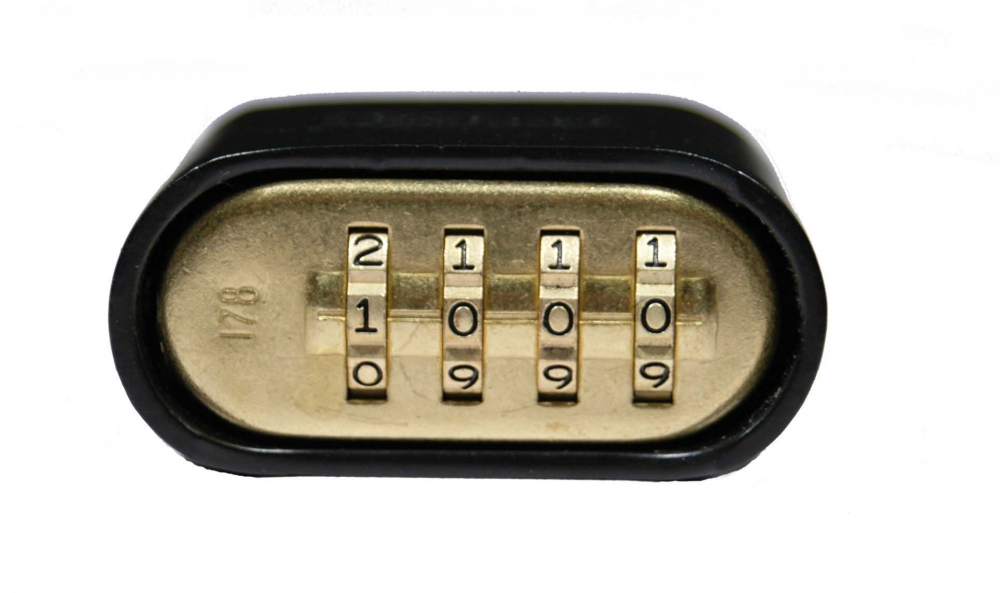
\includegraphics[scale=0.2]{gembok.png}
\end{center}

\textbf{Catatan}: Abaikan \textit{leading zero} atau digit $0$ yang berada diawal dalam membandingkan bilangan.

\subsection*{Format Masukan}
Baris pertama berisi bilangan bulat $T$ $(1 \leq T \leq 100)$, menyatakan banyaknya kasus uji.

Untuk setiap kasus uji, baris pertama berisi bilangan bulat $P$ $(1 \leq P \leq 10000)$, menyatakan panjang digit gembok

Kemudian baris berikutnya berisi $P$ digit angka $P_i$ $(0 \leq P_i \leq 9)$.

\subsection*{Format Keluaran}
Untuk setiap kasus uji ke-$i$, keluarkan satu baris yang berisi $P$ digit yang harus dimasukkan untuk membuka gembok Kurama.

\begin{multicols}{2}
\subsection*{Contoh Masukan}
\begin{lstlisting}
3
4
1234
5
11114
3
100

\end{lstlisting}
\columnbreak
\subsection*{Contoh Keluaran}
\begin{lstlisting}
0123
00003
001
\end{lstlisting}
\vfill
\null
\end{multicols}
\pagebreak
\subsection*{Penjelasan}
Penjelasan dari hasil keluaran adalah sebagai berikut:
\begin{itemize}
    \item Kasus ke-1 dapat dilakukan dengan menjumahkan semua digit dengan $1$ hingga muncul angka terkecil di setiap digitnya
    \item Kasus ke-2 menggunakan cara yang sama dengan kasus ke-1
    \item Kasus ke-3 dapat dilakukan dengan menggeser posisi digit kekiri, hingga didapat jawaban berupa bilangan terkecil
\end{itemize}
\pagebreak

\end{document}